%TC: macro \marginfootnote [other]
%TC: envir SCfigure [] other
%TC: macrocount beginSCfigure [figure]
\documentclass[11pt,twoside]{report}
\usepackage{preamble}
\setcounter{chapter}{2}
\graphicspath{{../img/}}
\def\includebibliography{}

\externaldocument{background}
\externaldocument{resummation}
\externaldocument{appendix-spt-singularities}

\begin{document}
\chapter{Many-body correlations from integral geometry}
\epigraph{Ninety percent of everything is crap.}{Theodore Sturgeon, \emph{Galaxy} (1956).}
\label{chapter:morphometric-framework}

%% This chapter will focus on the morphological framework for the treatment of many-body correlations.
%% This will cover two related topics:
%% \begin{enumerate}
%% \item \emph{Fundamental measure theory} which is ideally suited for correlations in Fourier space i.e.\ structure factors, and
%% \item The \emph{morphometric approach}, which presents a highly accurate alternative for real space calculations, albeit with many caveats.
%% \end{enumerate}
%% These two approaches are related in that they both depend on integral geometry, which we introduced in section \ref{sec:integral-geometry}.
%% In fact, we will see that the latter approach can be seen as a limiting case of the former.
%% We will focus on the theoretical developments in this chapter, and leave the main body of numerical work to the following chapter where we will apply this to local structure in the hard sphere liquid.

This chapter covers the theory for using morphological thermodynamics to treat many-body correlations inside the hard sphere liquid.
We introduced the morphometric approach in section \ref{sec:fmt} as a special case of fundamental measure theory, which is the traditional way it has been derived.
In this chapter we present the morphometric approach in a new context as a generalisation of scaled particle theory, and derive several morphometric theories for hard spheres of fundamental and practical interest.
Our central result will be a new theory which is particularly suited to the treatment of many-body correlation functions in the hard sphere liquid, which we demonstrate by numerical tests against simulation.
We leave applications of this framework to the next chapter.

Part of the work in this chapter is published in Ref.\ \cite{RobinsonPRL2019}, and the remaining parts will appear in a forthcoming paper \cite{RobinsonPRE2019}.

\section{Introduction}

Since the beginnings of modern liquid state theory \cite{KirkwoodJCP1935}, the hard sphere liquid has remained the archetypal model for atomic systems and soft matter.
The dynamics of the system at high density in the metastable regime above the freezing transition are hotly debated, despite relentless study.
%In particular, deep questions remain concerning its nucleation kinetics and dynamical arrest approaching the glass transition.
%Our central application will be to the treatment of many-body correlations in supercooled liquids, a potential new route for assessing causes of dynamical arrest.
Proposed mechanisms for dynamical phenomena all loosely fall under the broad umbrella of many-body correlations; nucleation occurs via crystal seed formation \cite{SearJPCM2007}, and to explain dynamic arrest approaching the glass transition thermodynamic theories invoke cooperatively rearranging regions \cite{LubchenkoARPC2007} or elastic soft modes \cite{BritoJCP2009} while kinetic theories posit the existence of dynamical defects \cite{ChandlerARPC2010}.
Here we propose a framework for treating many-body correlations, which in the next chapter we will develop into an operational scheme for predicting the populations and dynamics of local structural motifs within a uniform liquid.
Central to this is the use of the \emph{morphometric approach}.

The morphometric approach provides an efficient means of treating the thermodynamics of a bulk liquid without fully determining its equilibrium density profile \cite{KonigPRL2004,RothPRL2006,Hansen-GoosPRL2007,RobinsonPRL2019}.
Detailed investigations have shown that it is highly accurate in the hard sphere liquid regime \cite{OettelEL2009,AshtonPRE2011,LairdPRE2012,BlokhuisPRE2013,UrrutiaPRE2014,Hansen-GoosJCP2014}, so we can expect an accurate treatment where the bulk system provides background depletion interactions while its detailed microstates remain unimportant.
This feature makes it ideally suited for many-body correlations if we can identify relevant dynamical degrees of freedom.
While existing morphometric theories have been proven accurate in the liquid regime, we require a theory which works in the supercooled regime.
Here we derive such a theory using scaled particle theory (SPT).

SPT determines bulk properties from consideration of a spherical solute of varying radius.
It remains one of most enduring theories of simple liquids; though 60 years old as of this year \cite{ReissJCP1959}, aspects of this approach remain in modern theories.
This is particularly true for hard spheres where SPT has been unified with the Percus-Yevick integral equation solution \eqref{eq:pyc-pressure} \cite{WertheimPRL1963}, another old theory, in the form of fundamental measure theory (FMT) \cite{RosenfeldPRL1989} which we introduced in section \ref{sec:fmt}.
Though originally a theory of single-component hard spheres \cite{ReissJCP1959}, SPT has been extended to other potentials \cite{ReissJCP1960,HelfandJCP1960,ReissJCP1961} and shapes \cite{GibbonsMP1969,GibbonsMP1970}, mixtures \cite{LebowitzJCP1965}, dimers \cite{StillingerJCP2006,ChatterjeeJCP2006} and discs \cite{HelfandJCP1961,MartinJCP2018,Hansen-GoosJCP2019}.
Morphological thermodynamics can be seen as a modern generalisation of SPT for a wide class of physically relevant geometries.
Its basis in integral geometry replaces the semi-empirical approach of classical SPT with clearly defined postulates.
In this chapter we present the morphometric approach in the context of SPT and derive three theories for the single-component hard sphere liquid: the classical SPT coefficients, the White Bear II morphometric coefficients%
\marginfootnote{These are given in \eqref{eq:wbii-coefficients}, which we obtained through their classical derivation as part of FMT.
  In this chapter we will derive them through a new, self-contained route.}
and a new theory suitable for high densities above freezing.
%These extensions typically take a semi-empirical approach, and often the soundness of the assumptions are unclear.
%The virial expansion provides a few exact results which can be used to explore the limitations of approximate theories.

%% The morphometric approach can be seen as a limiting case of FMT, and this is more-or-less how specific theories have been derived \cite{Hansen-GoosJPCM2006}.
%% FMT was conceived as a unification of SPT and the Percus-Yevick integral equation solution for hard spheres \cite{WertheimPRL1963,LebowitzPR1964}, which resulted in the Rosenfeld functional \cite{RosenfeldPRL1989}.
%% SPT and the morphometric approach are obtained from the \emph{same} limit of FMT, so we can see the morphometric approach as a generalisation of SPT.
%% Furthermore, as limits of FMT it is tempting to analyse them within this more general framework.
%% However, we will find it instructive to study SPT/morphometry outside the context of FMT to incorporate more geometric intuition.
%% In addition, SPT is more flexible than FMT\todo{Rewrite this}: it has recently found use in hard discs where FMT fails \cite{MartinJCP2018,Hansen-GoosJCP2019}.

%% The seemingly unrelated Percus-Yevick correlation scaled particle and the theories approximation to the direct correlation for \emph{homogeneous} hard spheres were unified by Rosenfeld into a theory for \emph{inhomogeneous} fluids creating FMT \cite{RosenfeldPRL1989}.

%Although FMT supercedes SPT, it is instructive to revisit a purely SPT approach to develop a deeper understand of the foundations of the morphometric approach as well as its limitations.

%Summary of literature:
%% \begin{itemize}
%% \item Original for hard spheres: \cite{ReissJCP1959}
%% \item Extension to real fluids \cite{ReissJCP1960,HelfandJCP1960,ReissJCP1961}
%% \item Hard discs \cite{HelfandJCP1961}, \cite{MartinJCP2018,Hansen-GoosJCP2019}.
%% \item Inclusion of non-morphological terms by expanding in a Laurent series \cite{MandellJSP1976}, scaling with a fractional power: \cite{Hansen-GoosJCP2019}
%% \item Simplified treatment including mixtures \cite{LebowitzJCP1965}
%% \item Nonspherical convex particles \cite{GibbonsMP1969}.
%% \item Mixtures of nonspherical convex particles \cite{GibbonsMP1970}.
%% \item More recently hard sphere pairs in \cite{StillingerJCP2006,ChatterjeeJCP2006}.
%% \end{itemize}
%% \hl{Other literature we should cite: Refs} \cite{FrischAiCP1964,ReissAiCP1965,ReissJCP1974,Tully-SmithJCP1970,HarrisJCP1971}.
%% Not SPT: PY solution for mixtures of hard spheres \cite{LebowitzPR1964}.

%% For hard interactions these integrals are known to reduce to a particularly simple form in terms of the morphological measures of each body, which we will describe below in detail.
%% Mention one of the reasons for this is to develop a clear criterion for the validity of geometric approach: choice of dividing surface, valid geometries (no self-intersection).

In section \ref{sec:many-body-correlations} we show how one can map the problem of treating many-body correlations onto a solvent-solute problem.
We spend the rest of the chapter discussing the solvation problem through the lens of SPT.
We argue for the morphometric approach as a useful generalisation of SPT in section~\ref{sec:morphometric-approach}.
Then, through scaled particle arguments for hard spheres, we derive the classical SPT theory, the White Bear II morphometric theory \cite{Hansen-GoosJPCM2006} and a new set of coefficients well-suited for treating many-body correlations.
In section \ref{sec:numerics} we numerically test these theories' two-- and three--body correlation functions to demonstrate their effectiveness in treating correlation functions.
%The latter coefficients were first derived in the Supplementary Material of our earlier work \cite{RobinsonPRL2019}, and aim to give them a complete account here.

\section{Solvation expression for many-body correlations}
\label{sec:many-body-correlations}

\subsection{Correlations in terms of the insertion cost}

We will show that correlations of $n$ particles at positions $\vec{r}^n := \{\vec{r}_1, \cdots, \vec{r}_n\}$ can be expressed in terms of the free energy cost of inserting them at $\vec{r}^n$, by generalising the \emph{potential distribution theorem} \cite{WidomJCP1963,WidomJPC1982} to many particles.
The classical approach, also known as \emph{Widom's insertion method}, expresses the (excess) chemical potential $\mu^\mathrm{ex}$ of a single-component system as the free energy cost of inserting an additional particle.
See Ref.\ \cite{Rowlinson2002} and references therein for a detailed review of this classical approach.
Our generalisation results in a \emph{potential of mean force} for interactions between the $n$ particles, which is formally identical to the chemical potential of a solute; this latter form is particularly suitable for geometric approximation schemes.

We consider a bulk liquid (the solvent) of $N$ particles with interaction potential energy $U_N$ surrounding the $n$ particles (the solute).
To coarse-grain onto the $n \ll N$ degrees of freedom we must perform an average over all arrangements of this solvent.
Specifically, we will describe many-body correlations with the $n$-particle density defined in \eqref{eq:n-particle-density-pdf}; the specific form for grand-canonical ensemble is given already in \eqref{eq:n-particle-density} but we restate it here for ease of reference:
\begin{equation*}
  \rho^{(n)}(\vec{r}^n)
  =
  \frac{1}{\Xi} \sum_{N=n}^\infty \frac{z^N}{(N-n)!} \int e^{-\beta U_N} \, d\vec{r}^{(N-n)}.
\end{equation*}
Changing the summation limits $N \rightarrow N+n$ we obtain
\begin{equation}\label{eq:n-particle-density-term-separation}
\begin{aligned}
  \rho^{(n)}(\vec{r}^n)
  &=
  \frac{z^n}{\Xi} \sum_{N=0}^\infty \frac{z^N}{N!} \int e^{-\beta U_{N+n}} \, d\vec{r}^{N}
  \\ &=
  z^n e^{-\beta U_n} \left< e^{-\beta U_{n \leftrightarrow N}} \right>
\end{aligned}
\end{equation}
where in the latter step we decomposed the total potential $U_{N+n}$ into purely local and solvent terms, i.e.\ $U_{N+n} = U_n + U_N + U_{n \leftrightarrow N}$, where $U_\alpha$ for $\alpha \in \{n,N\}$ indicates the internal interactions between particles in component $\alpha$.
The ``interspecies'' interactions are contained within $U_{n \leftrightarrow N}$ which acts as an external field for the solvent.
Thus, \eqref{eq:n-particle-density-term-separation} becomes
\begin{equation*}
  \rho^{(n)}(\vec{r}^n)
  =
  z^n e^{-\beta (U_n + \Omega - \Omega_\mathrm{hom})}.
\end{equation*}
where $\Omega$ is the grand potential of the solvent in the presence of the $n$-particle inhomogeneity.
Splitting the chemical potential into its ideal and excess parts so that $\beta\mu = \ln{\Lambda^d \rho} + \beta\mu^\mathrm{ex}$ gives
\begin{equation*}
  \rho^{(n)}(\vec{r}^n)
  =
  \rho^n e^{-\beta (U_n + \Omega - \Omega_\mathrm{hom} - n\mu^\mathrm{ex})}.
\end{equation*}
The $n$-particle distribution functions are then determined from \eqref{eq:n-particle-distribution}
\begin{equation}\label{eq:distribution-solvation}
  g^{(n)}(\vec{r}^n)
  := \frac{\rho^{(n)}(\vec{r}^n)}{\rho^n}
  = e^{-\beta(U_n + \Delta\Omega - n\mu^\mathrm{ex})}
\end{equation}
where $\Delta\Omega := \Omega - \Omega_\mathrm{hom}$ is the reversible (free energy) cost of inserting the particles at fixed position $\vec{r}^n$, or equivalently describes the average depletion interactions between mobile particles.
For $n=1$ we have $\Delta\Omega = \mu^\mathrm{ex}$ and this is identical to the potential distribution theorem of Widom \cite{WidomJCP1963,WidomJPC1982}.
The distribution functions are written in terms of the potential
\begin{equation}\label{eq:potential-mean-force}
  \begin{split}
    \phi^{(n)}(\vec{r}^n) &:=
    - k_B T \ln{g^{(n)}(\vec{r}^n)} \\
    &=
    U_n + \Delta\Omega - n\mu^\mathrm{ex},
  \end{split}
\end{equation}
which we call the \emph{generalised potential of mean force}.
For the case $n=2$ this reduces to the usual potential of mean force in the liquid state literature \cite{Hansen2013}.

This completes our proof that the correlations can be transformed to a potential, and we can proceed with a geometrical construction for $\Delta \Omega$.

\begin{SCfigure}
  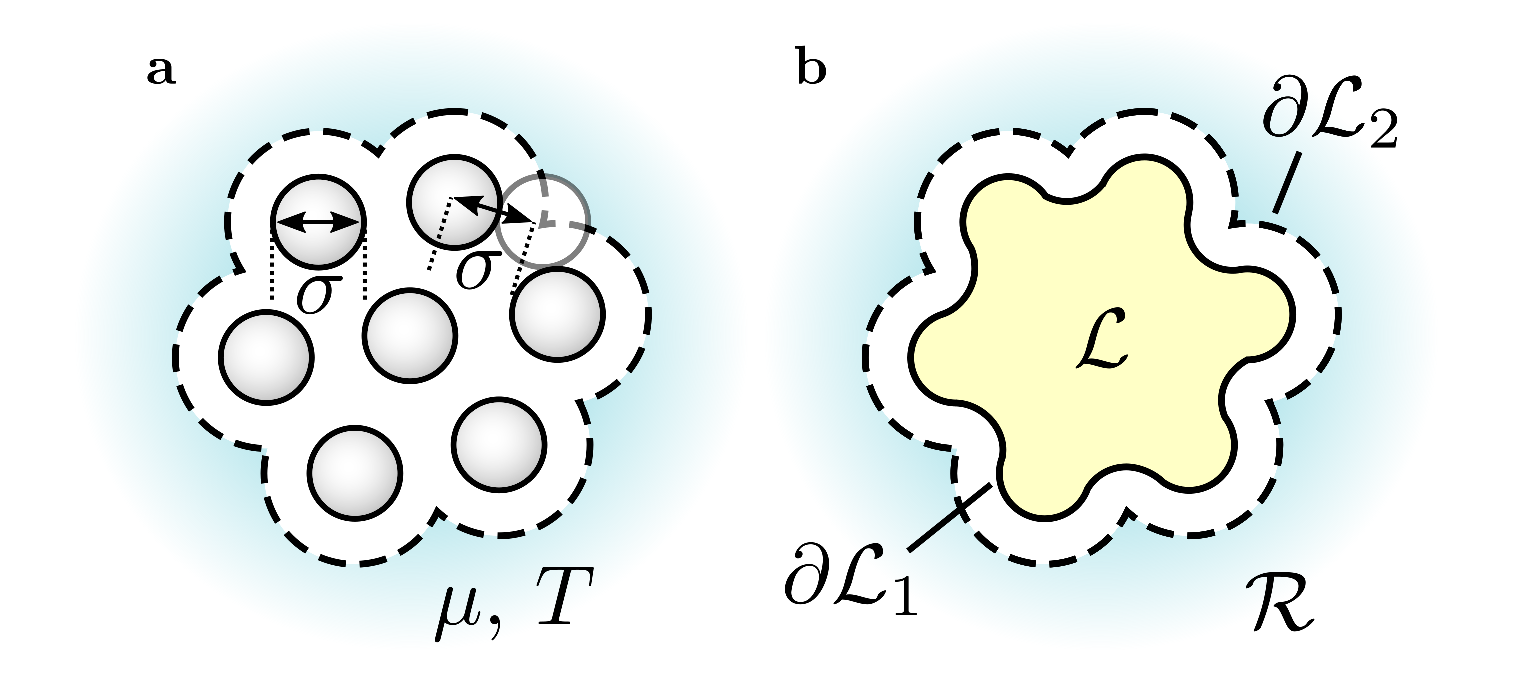
\includegraphics[width=\linewidth,outer]{morph-droplet}
  \caption[Our system: correlations as solvation physics]{
    The system considered for many-body correlations showing
    (a) the local particles surrounded by the remaining liquid acting as a thermal reservoir at fixed chemical potential and temperature, and
    (b) possible partitions of space into the local $\mathcal{L}$ and remaining $\mathcal{R}$ components for two choices of dividing surface: $\partial\mathcal{L}_1$ is the molecular surface while $\partial\mathcal{L}_2$ is the solvent accessible surface (see discussion around Eq.\ \eqref{eq:exclusion-transform}).
  }
  \label{fig:system}
\end{SCfigure}

%% Before moving on, we comment on extensions of the above result:
%% \begin{itemize}
%% \item \emph{Mixtures}: repeating the steps in the derivation of \eqref{eq:distribution-solvation} and \eqref{eq:potential-mean-force} to an $m$-component mixture gives a potential of mean force which is nearly identical
%%   \begin{equation*}
%%     \begin{split}
%%       \phi^{(\{n_i\})}(\vec{r}^n) &:=
%%       - k_B T \ln{g^{(n)}(\vec{r}^n)} \\
%%       &=
%%       U_n + \Delta\Omega - \sum_{i=1}^m n_i \mu_i^\mathrm{ex},
%%     \end{split}
%%   \end{equation*}
%%   where the tuple $\{n_1, \cdots, n_m\}$ gives the number of each species of particle with $n = \sum_{i=1}^m n_i$, and $\mu_i^\mathrm{ex}$ as the excess chemical potential of species $i$.
%% \item \emph{Many-body interactions}: for more complicated interaction potentials (i.e.\ beyond pair potentials) \eqref{eq:distribution-solvation} and \eqref{eq:potential-mean-force} are still correct but the decomposition between internal interactions and grand potential is not as clean.
%%   For example, consider a system interacting with an additional three-body potential $u_{i,j,k}$.
%%   In addition to a contribution to $U_{n \leftrightarrow N}$ which acts as an effective external field, a term develops which includes interactions between \emph{two} solvent particles and each solute particle:
%%   \begin{equation*}
%%     \begin{split}
%%     U_{n \leftrightarrow N}
%%     =& \phantom{+}
%%     \sum_{k=n+1}^{N} \underbrace{\sum_{i=0}^n \left( u_{i,j} + \sum_{j=0}^n u_{i,j,k} \right)}_\textrm{effective external field}
%%     \\ & +
%%     \sum_{n < i < j} \left( \sum_{k = 0}^n u_{i,j,k} \right).
%%     \end{split}
%%   \end{equation*}
%%   The latter term acts as an effective pair potential between $i$ and $j$, so
%%   the inhomogeneity can be thought of as perturbing the pair-potential of the surrounding liquid and $\Delta\Omega$ must reflect this change.
%% \end{itemize}

\subsection{Representing the insertion cost as a solvation problem}
\label{sec:insertion-as-solvation}

For systems with excluded volume interactions, we can divide the space into a local component $\mathcal{L} \subset \mathbb{R}^d$ of volume $V_\mathcal{L}$ inaccessible to solvent degrees of freedom and the remaining space $\mathcal{R} = \mathbb{R}^d \setminus \mathcal{L}$ of volume $V_\mathcal{R}$ filled by the rest of the liquid (Fig. \ref{fig:system}).
The total volume is $V = V_\mathcal{L} + V_\mathcal{R}$ so the homogeneous grand potential is
\begin{equation*}
  \Omega_\mathrm{hom} = -p V.
\end{equation*}
After inserting the inhomogeneity the total volume accessible to the rest of the liquid will be reduced by $V_\mathcal{L}$, so the grand potential becomes
\begin{equation*}
  \Omega = -p V_\mathcal{R} + \Omega_\mathrm{ex}[\partial\mathcal{L}],
\end{equation*}
where $\Omega_\mathrm{ex}$ is an excess term brought about by the introduction of a dividing surface $\partial\mathcal{L}$ between the two liquid components.
Subtracting these two expressions gives
\begin{equation*}
  \Delta \Omega
  := \Omega - \Omega_\mathrm{hom}
  = p V_\mathcal{L} + \Omega_\mathrm{ex}[\partial\mathcal{L}].
\end{equation*}
This dividing surface has area $A_{\partial\mathcal{L}}$, creating a surface tension $\gamma$ so we can write the excess term as
\begin{equation*}
  \Omega_\mathrm{ex}[\partial\mathcal{L}] =
  \gamma[\partial\mathcal{L}] A_{\partial\mathcal{L}}
\end{equation*}
which is a formal definition of surface tension and depends on the choice of dividing surface (see two examples in Fig.\ \ref{fig:system}(b)).
We know from density functional theory \cite{EvansAP1979} that the excess free energy is a functional of the density profile, which will in turn depend on the shape of the boundary; we write $\gamma = \gamma[\partial \mathcal{L}]$ to indicate this functional dependence on the surface shape.
The \emph{solvation form} of the inhomogeneous grand potential term in \eqref{eq:potential-mean-force} is then
\begin{equation}\label{eq:surface-tension}
  \Delta \Omega[\mathcal{L}] =
  p V_\mathcal{L} + \gamma[{\partial\mathcal{L}}] A_{\partial\mathcal{L}}.
\end{equation}
The problem of determining the $n$-particle distributions has been reduced to a solvation problem: we must find the surface tension between a solute (the specific local arrangement) and a solvent (the rest of the liquid).
We will use the solute--solvent terminology, but one could also think of local--bulk nomenclature.

\section{Scaled particle ansatz}
\label{sec:morphometric-approach}

In every formulation of scaled particle theory one considers a hard \emph{spherical} solute of radius $R$.
In most approaches, the cost $\Delta \Omega$ is assumed to have an analytic expansion in powers of the radius; in classical approaches this was simply postulated, however we will be able provide proper justification below through geometric arguments.
Recognising that terms scaling faster than $R^3$ must be zero for it to remain well-defined in the limit of large solutes leads to the third order polynomial \cite{ReissJCP1959}
\begin{equation}\label{eq:spt-ansatz}
  \Delta\Omega(R) =
  p \, \frac{4\pi R^3}{3} + a_2 \, 4 \pi R^2 + a_1 \, 4 \pi R + a_0 \, 4 \pi,
\end{equation}
where we identified the largest power with the work term $pV$ from comparison with \eqref{eq:surface-tension}, and $\{a_0, a_1, a_2\}$ are thermodynamic coefficients describing the subleading corrections.
We have chosen to introduce factors of $4\pi$ in front of subleading terms to suggest how we will generalise beyond spherical geometries; these are normalisations of the intrinsic volumes, as can be seen by comparison with table \ref{table:geometric-quantities}.
Specifically, these terms can be identified with the volume, surface area, and integrated mean and Gaussian curvatures.
For a general solute $K \subset \mathbb{R}^3$ we then write the morphometric insertion cost as%
\marginfootnote{This \emph{ansatz} is identical to the result we obtained as a limit of FMT in \eqref{eq:fmt-morphometric-2}, up to different normalisations of the intrinsic volumes.
  We will not emphasise this point, as our intent is to develop the ideas independent of FMT with the goal of arriving at a more flexible theory which can be specialised to the correlation functions.}
\begin{equation}\label{eq:morph-ansatz}
  \Delta\Omega[K] =
  p V[K]
  + a_2 A[K]
  + a_1 C[K]
  + a_0 X[K].
\end{equation}
%where $C$ and $X$ are the integrated mean and Gaussian curvatures.
All of these functionals act on $K$ but the latter three can also be \emph{expressed} as surface integrals, as given by \eqref{eq:intrinsic-volumes-surface-integrals}.
For a spherical solute these reduce to the values given in \eqref{eq:spt-ansatz}, so this represents a proper generalisation of SPT for more general geometries.

We now give a brief justification of the above \emph{ansatzes}, in particular why there are only four terms in the expansion.
Radius is the only natural parameter for a sphere, however for more general geometries there might be arbitrarily many parameters so one may wonder if they should be included in a general geometric expansion.
Nevertheless, we can make compelling arguments using integral geometry, introduced in section \ref{sec:integral-geometry}, to only retain the terms listed.
Most notably, the terms included are the \emph{only} physically meaningful size measures (cf.\ section \ref{sec:what-is-size}), and so $\Delta \Omega$ is strictly extensive if it is a linear combination of these measures%
\marginfootnote{See discussion on extensivity and references cited around equations \eqref{eq:extensive-homogeneity} and \eqref{eq:extensive-integral-geometry}, as well as Hadwiger's theorem \eqref{eq:extensive-integral-geometry-d}.}.
This argument was first applied to hard sphere solvation in Ref.\ \cite{KonigPRL2004}.

The central assertion of the morphometric approach is that the insertion cost $\Delta \Omega$ \emph{exactly} possesses the properties above, providing the connection between geometry and thermodynamics \cite{KonigPRL2004}.
The morphometric form \eqref{eq:morph-ansatz} then follows.
In addition to providing a more general \emph{ansatz} than SPT, this approach lays out its underlying assumptions explicitly eschewing the ad-hoc way in which the original SPT \emph{ansatz} \eqref{eq:spt-ansatz} was obtained.
Moreover, classical SPT assumes hard spheres from the outset while our generalisation based on integral geometry is more flexible, allowing for generalisations to mixtures, more realistic pair potentials and non-spherical particles without compromising its assumptions.

The morphometric approach is certainly an approximation, as the insertion cost will not rigorously possess the properties of size measures in reality.
Notably, in SPT $\Delta\Omega$ is known to contain singularities in its high order derivatives with solute radius%
\marginfootnote{We review the original argument for this from Ref.\ \cite{ReissJCP1959} in Appendix \ref{appendix:spt-singularities}.
This argument is quite general, demonstrating that \emph{any} analytic form of $\Delta \Omega$ in terms of geometric quantities cannot be exact.};
these non-analytic terms result from violations of the additivity assumption.
Nevertheless, the approximation is accurate in hard spheres \cite{OettelEL2009,AshtonPRE2011,LairdPRE2012,BlokhuisPRE2013,UrrutiaPRE2014,Hansen-GoosJCP2014} so these violations should be small.

%% The connection between intrinsic volumes and thermodynamics was made by K\"onig et al \cite{KonigPRL2004}.
%% They argued that $\Delta \Omega$ possesses all three properties above, so it must be expressable as a linear sum of the volumes $\{V_k\}$ through the theorem of Hadwiger \cite{Hadwiger1957}.
%% In this case we say that the insertion cost of a solute $K$ is of \emph{morphometric form} and can be written as
%% \begin{equation}\label{eq:morph-ansatz}
%%   \Delta \Omega[K] = \sum_{k=0}^d a_k V_k(K)
%% \end{equation}

%% Given the plausibilty of the rigid-motion invariance and continuity, additivity is the most highly restrictive condition on $\Delta \Omega$.
%% In section~\ref{sec:finite-densities} we obtain a contribution to the insertion cost which \emph{is} strictly additive, but it is not the only term in $\Delta\Omega$ except in limiting cases which we will discuss in subsequent sections.
%% %Additionally, for soft interaction potentials we do not expect it to hold exactly in any limit.
%% On the other hand, additivity implies extensivity and on thermodynamic grounds we generally expect extensivity to hold for very large objects; as such, it is plausible for additivity to hold in general in the limit of large solutes.
%% Nevertheless, there is much evidence that the additivity assumption is not exact in hard spheres
%% \cite{LairdPRE2012,BlokhuisPRE2013,UrrutiaPRE2014,Hansen-GoosJCP2014}.
%% In particular, comparison of the cluster expansion of $\Delta \Omega$ for spheres and cylinders shows unambiguous deviations from morphometric form which do not disappear in the large solute limit \cite{UrrutiaPRE2014}.
%% These deviations were found to be small for hard spheres, so while approximate it seems to be a useful assumption.

\section{Obtaining thermodynamic coefficients}
\label{sec:spt}

We will consider a single-component hard sphere fluid, for particles of diamter $\sigma$ and bulk volume fraction $\eta$.
We will take the morphometric \emph{ansatz} \eqref{eq:morph-ansatz} and obtain coefficients for this system using scaled particle arguments.
However, unlike the classical arguments this \emph{ansatz} is more general in its scope; we will exploit this feature of the morphometric approach to construct new theories suitable for the treatment of many-body correlations with high accuracy.
Before we obtain new coefficients we will rederive the classical SPT and the White Bear II coefficients.
The latter set of coefficients was originally obtained as a limiting case of FMT \cite{Hansen-GoosJPCM2006}; here we obtain them through purely scaled particle arguments, which lays the groundwork for construction of the new coefficients.

All coefficients we give are for the molecular geometry bounded by the \emph{molecular surface} ($\partial \mathcal{L}_1$ in Fig.\ \ref{fig:system}b), the surface where interactions occur between the solute and a test particle representing the remaining liquid.
However, it is usually more convenient to do calculations with the excluded geometry: the space inaccessible to the \emph{center} of a test particle bounded by the \emph{solvent accessible surface} ($\partial \mathcal{L}_2$ in Fig.\ \ref{fig:system}b).
The original definitions of these surfaces can be found in Refs.\ \cite{LeeJMB1971,RichardsARBB1977}.
Note that there is also an infinite family of well-defined parallel surfaces between these two extremes, but they are not widely used in practice so we will not consider them \cite{OettelEL2009}.
The choice of dividing surface will change the surface tension, and thus requires new coefficients $\{a_0', a_1', a_2'\}$ i.e.\
\begin{equation}
  \Delta\Omega[K]
  =
  p V_+[K]
  + a_2' A_+[K]
  + a_1' C_+[K]
  + a_0' X_+[K],
\end{equation}
where the excluded geometry terms transform via the canonical relations \cite{Hansen-GoosJPCM2006,OettelEL2009,Santalo2004,Klain1997}
\begin{subequations}\label{eq:exclusion-transform-volumes}
  \begin{align}
    X_+[K]
    &=
    X[K],
    \\
    C_+[K]
    &=
    C[K] + \frac{\sigma}{2} X[K],
    \\
    A_+[K]
    &=
    A[K] + \sigma C[K] + \frac{\sigma^2}{4} X[K],
    \\
    V_+[K]
    &=
    V[K]
    + \frac{\sigma}{2} A[K]
    + \frac{\sigma^2}{4} C[K]
    + \frac{\sigma^3}{24} X[K].
  \end{align}
\end{subequations}
%$+$-subscripts on the geometric terms indicate that they are for the exclusion geometry.
It is straightforward to transform between these two conventions via \cite{Hansen-GoosJPCM2006,OettelEL2009}
\begin{subequations}\label{eq:exclusion-transform}
  \begin{align}
    a_0'
    &=
    a_0
    - \frac{\sigma}{2} a_1
    + \frac{\sigma^2}{4} a_2
    - \frac{\sigma^3}{24} p,
    \\
    a_1'
    &=
    a_1
    - \sigma a_2
    + \frac{\sigma^2}{4} p,
    \\
    a_2'
    &=
    a_2 - \frac{\sigma}{2} p.
  \end{align}
\end{subequations}
The resulting $\Delta \Omega$ will be identical whichever surface is chosen, except when there is a topological change in the molecular surface marking the breakdown of the theory; this is discussed in detail in Ref.\ \cite{OettelEL2009}.

A crucial component of scaled particle approaches is thermodynamic consistency of the (osmotic) pressure \eqref{eq:consistent-osmotic-pressure} which we restate here as%
\marginfootnote{We remind the reader that $f^\mathrm{ex} = F^\mathrm{ex}/V$ is the (excess) free energy density.}
\begin{equation}\label{eq:osmotic-consistency-1}
  \beta p
  =
  \rho - \beta f^\mathrm{ex}
  + \rho \left( \frac{\partial \beta f^\mathrm{ex}}{\partial \rho} \right)_{V,T}.
\end{equation}
The form most useful for a single-component system comes from taking the derivative with respect to density, and noting the definition of the excess chemical potential
\begin{equation*}
  \beta \mu^\mathrm{ex}
  =
  \left( \frac{\beta f^\mathrm{ex}}{\partial \rho} \right)_{V,T},
\end{equation*}
giving
\begin{equation}\label{eq:osmotic-consistency-2}
  %\begin{split}
    \left( \frac{\partial \beta p}{\partial \rho} \right)_{V,T}
    %&=
    =
    \rho \left( \frac{\partial \beta \mu}{\partial \rho} \right)_{V,T}
    %\\
    =
    1 + \rho \left( \frac{\partial \beta \mu^\mathrm{ex}}{\partial \rho} \right)_{V,T}.
  %\end{split}
\end{equation}
Note that the consistency relation \eqref{eq:osmotic-consistency-1} provides the route to generalising all of our arguments to arbitrary mixtures \cite{RosenfeldPRL1989,SollichAiCP2001,SantosPRE2012}.
As we discussed in \ref{sec:truncatable-free-energy}, the free energy remains well-defined for polydisperse mixtures if the composition dependence enters only through a set of weighted moments of the density $\{\xi_k\}$.
Then \eqref{eq:osmotic-consistency-1} becomes
\begin{equation}\label{eq:osmotic-consistency-3}
  \beta p
  %% &=
  %% \rho - \beta f^\mathrm{ex}
  %% + \rho \left( \frac{\partial \beta f^\mathrm{ex}}{\partial \rho} \right)_{V,T}
  %% \\ &=
  =
  \rho - \beta f^\mathrm{ex}
  + \sum_k
  \xi_k \left( \frac{\partial \beta f^\mathrm{ex}}{\partial \xi_k} \right)_{V,T}.
\end{equation}
For weighted densities consistent with an SPT (or FMT) approach, it has been shown Ref.\ \cite{SantosPRE2012} that the thermodynamic coefficients for mixtures are determined once an equation of state for the single-component system is known.

\subsection{Classical scaled particle relations}
\label{sec:classical-spt}

\begin{SCfigure}
  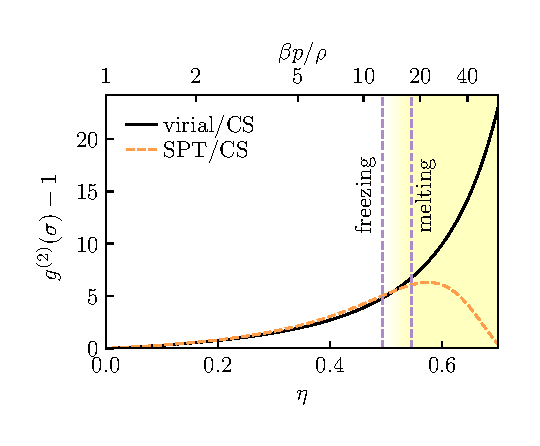
\includegraphics[width=0.9\linewidth,outer]{g2-contact}
  \caption[Contact values of pair distribution function $g^{(2)}(r)$]{
    Contact values of the radial distribution function against volume fraction $\eta$ and reduced pressure for the hard sphere liquid using \eqref{eq:contact-g} with \eqref{eq:distribution-solvation} and \eqref{eq:morph-ansatz} for the explicit form of $g^{(2)}$, assuming the Carnahan-Starling (CS) equation of state.
    Contact values are determined with two sets of morphometric coefficients: SPT/CS (section \ref{sec:cs-spt}, specifically \eqref{eq:cs-spt-coefficients}, or equivalently the White Bear II bulk coefficients \eqref{eq:wbii-coefficients} of Ref.\ \cite{Hansen-GoosJPCM2006}) which performs poorly in the supercooled regime (shaded area), and coefficients derived in this chapter (section \ref{sec:virial-spt}) using the virial theorem which is exact by construction.
    The hard sphere freezing and melting volume fractions are indicated by purple dashed lines to show the onset of the supercooled regime.
  }
  \label{fig:contact-g}
\end{SCfigure}

The key advantage of a geometric expansion of the free energy is that the role of thermodynamics and geometry are kept separate.
Thermodynamics only enters through the coefficients $\{p,a_2,a_1,a_0\}$, so they can be determined in simple geometries to obtain a general theory.
After determining these coefficients all the complexity of computing $\Delta \Omega$ is reduced to measuring the geometric quantities $\{V,A,C,X\}$ of the specific solute.

Following the protocol of scaled particle theories, we consider the insertion of a hard spherical solute of radius $R$ into the liquid.
Assuming the morphometric form for the insertion cost returns us to the \emph{ansatz} \eqref{eq:spt-ansatz}.
The approximate theory is linear so we need \emph{only} 4 equations to set the thermodynamic coefficients.
With many thermodynamic relations to choose from the theory is overconstrained in general.
We must use physical intuition to choose suitable equations, after which the accuracy of the resulting coefficients can be assessed.
Below we give the exact thermodynamic relations for hard spheres which produce the classical SPT coefficients.

It is possible to consider the insertion of a solute with a \emph{negative} radius: the hard core interaction between the two particles only occurs when the solute is `inside' a solvent particle.
In this limit the insertion cost can be determined exactly as \cite{ReissJCP1959}
\begin{equation}
  \beta \Delta \Omega =
  -\ln{\left(
    1 - \frac{4\pi \left(R + \frac{\sigma}{2}\right)^3}{3} \rho
    \right)}
\end{equation}
for $-\frac{\sigma}{2} \le R \le 0$.
It may appear concerning that this result does not possess the morphometric form \eqref{eq:morph-ansatz}; however, this does not discount the validity of the morphometric approach as the nonphysical geometry violates the continuity assumption (section~\ref{sec:morphometric-approach}) because it cannot be approximated by polyhedra.
This places the result for $R < 0$ outside the theory's stated regime of validity, however $\Delta\Omega$ is continuous up to its second derivative across $R=0$ with a discontinuity in its third derivative \cite{ReissJCP1959}.
In the limit $R \to 0$ the expression above corresponds to the cost of inserting a hard point giving
\begin{subequations}\label{eq:spt-origin-continuity}
  \begin{align}
    \label{eq:spt-point}
    \beta \Delta\Omega(R=0)
    &=
    -\ln{(1- \eta)},
    \\
    \label{eq:spt-point-d1}
    \beta \left. \left(
    \frac{\partial \Delta\Omega}{\partial R}
    \right)_{\mu, V, T} \right|_{R=0}
    &=
    \frac{6\eta}{\sigma (1- \eta)},
    \\
    \label{eq:spt-point-d2}
    \beta \left. \left(
    \frac{\partial^2 \Delta\Omega}{\partial R^2}
    \right)_{\mu, V, T} \right|_{R=0}
    &=
    \frac{12\eta^2 + 24\eta}{\sigma^2 (1- \eta)^2}.
 \end{align}
\end{subequations}
Note that \eqref{eq:spt-point} can also be justified by considering that the probability of a randomly selected position in space being empty is simply the free volume $1-\eta$.

Together applying \eqref{eq:spt-origin-continuity} to \eqref{eq:spt-ansatz} fixes the coefficients $\{a_0, a_1, a_2\}$, so the theory requires an additional thermodynamic relation to determine the pressure.
When $R = \frac{\sigma}{2}$ the solute is equivalent to the solvent particles themselves and we recover $\Delta\Omega = \mu^\mathrm{ex}$, so from \eqref{eq:spt-ansatz} we have
\begin{equation}\label{eq:spt-mu}
  \Delta\Omega\left(R=\frac{\sigma}{2}\right) =
  \frac{\pi \sigma^3}{6} p
  + \pi \sigma^2 \, a_2
  + 2 \pi \sigma \, a_1
  + 4\pi \, a_0
  =
  \mu^\mathrm{ex}.
\end{equation}
Combining this expression with the thermodynamic relation \eqref{eq:osmotic-consistency-2} gives a differential equation for $\beta p$ whose solution gives the classical SPT coefficients for hard spheres as \cite{ReissJCP1959,LebowitzJCP1965}
\begin{subequations}\label{eq:py-coefficients}
  \begin{align}
    \beta a_0^\mathrm{SPT/PY}
    &=
    -\frac{\ln{(1- \eta)}}{4\pi},
    \\
    \beta a_1^\mathrm{SPT/PY}
    &=
    \frac{3\eta}{2\pi \sigma (1 - \eta)},
    \\
    \beta a_2^\mathrm{SPT/PY}
    &=
    \frac{6\eta + 3\eta^2}{2\pi \sigma^2 (1 - \eta)^2},
    \\
    \frac{\beta p^\mathrm{SPT/PY}}{\rho}
    &=
    \frac{1 + \eta + \eta^2}{(1 - \eta)^3}.
    \label{eq:py-pressure}
 \end{align}
\end{subequations}
The equation of state \eqref{eq:py-pressure} is equivalent to the one obtained through the solution of the Percus-Yevick (PY) integral equation%
\marginfootnote{See section \ref{sec:fmt} and Ref.\ \cite{WertheimPRL1963}.};
these two routes have been unified within FMT as the Rosenfeld functional \eqref{eq:rosenfeld-functional} \cite{RosenfeldPRL1989} which we have already seen produces \emph{identical} coefficients in the bulk limit \eqref{eq:rosenfeld-coefficients}.

Before we move on to generalisations of SPT, we will review one more thermodynamic relation which is satisfied by the classical solution \eqref{eq:py-coefficients}.
This emphasises the remarkable degree of self-consistency of SPT, and the additional relation will be used to construct new theories in subsequent sections.

We can relate the radial derivative of $\Delta\Omega(R)$ to the solvent density at contact; by connecting this to the virial theorem we can obtain a new thermodynamic relation.
Following Ref.\ \cite{BrykPRE2003} we take the normal derivative of $\Omega$ with respect to $R$, and noting that $\Delta\Omega(R) = \Omega(R) - \Omega_\mathrm{hom}$ gives
\begin{equation}\label{eq:spt-derivative}
  \begin{split}
    \left( \frac{\partial \Delta \Omega}{\partial R} \right)_{\mu,V,T}
    =&
    \left( \frac{\partial \Omega}{\partial R} \right)_{\mu,V,T}
    \\ =&
    \int
    \frac{\delta \Omega[\rho^{(1)}(\vec{r})]}{\delta \rho}
    \left( \frac{\partial \rho^{(1)}(\vec{r})}{\partial R} \right)_{\mu,V,T}
    \, d\vec{r}
    \\ &
    + \int
    \rho^{(1)}(\vec{r})
    \left( \frac{\partial \phi_\mathrm{ext}(\vec{r}; R)}{\partial R} \right)_{\mu,V,T}
    \, d\vec{r},
  \end{split}
\end{equation}
where $\phi_\mathrm{ext}$ is the external potential (i.e.\ the potential of the solute).
As a reminder, we defined $\rho^{(1)}$ as the equilibrium density profile in \eqref{eq:single-particle-density}.
In equilibrium $\Omega$ is minimised \eqref{eq:dft-equilibrium} so the first integral in \eqref{eq:spt-derivative} vanishes.
As the solute is hard, the external potential and its derivative are zero everywhere except at a distance $\frac{\sigma}{2}$ from the surface where both $\rho^{(1)}$ and $\phi_\mathrm{ext}$ are discontinuous.
We consider its Boltzmann weight, i.e.\
\begin{equation*}
  e^{-\beta\phi_\mathrm{ext}(\vec{r})}
  =
  \Theta\left( |\vec{r}| - R - \frac{\sigma}{2} \right).
\end{equation*}
Taking the (distributional) derivative of both sides gives
\begin{equation*}
  \beta\left( \frac{\partial\phi_\mathrm{ext}(\vec{r})}{\partial R} \right)_{\mu,V,T}
  =
  \delta\left( |\vec{r}| - R - \frac{\sigma}{2} \right)
  e^{\beta\phi_\mathrm{ext}(\vec{r})}.
\end{equation*}
Inserting this expression into \eqref{eq:spt-derivative} and using the fact that $\rho^{(1)}(\vec{r}) e^{\beta\phi_\mathrm{ext}(\vec{r})}$ is a continuous function (cf.\ Ref.\ \cite{Hansen2013}) gives the contact theorem
\begin{equation*}
  \beta \left( \frac{\partial \Omega}{\partial R} \right)_{\mu,V,T}
  =
  4\pi \left( R + \frac{\sigma}{2} \right)^2
  \rho^{(1)}\left( R + \frac{\sigma}{2} \right)
\end{equation*}
and the contact density in this inhomogeneous system is $\rho^{(1)}(\sigma; \phi_\mathrm{ext}) := \rho^{(2)}(\sigma)/\rho = \rho \, g^{(2)}(\sigma)$ recalling the definition of $\rho^{(n)}$ for the homogeneous system%
\marginfootnote{This is argument, due to Percus \cite{PercusPRL1962}, is ordinarily used to construct integral equation theories based around the Ornstein-Zernike equation \eqref{eq:ornstein-zernike-spherical} (cf.\ Ch.\ 4 of Ref.\ \cite{Hansen2013}).}
\eqref{eq:n-particle-density-pdf}, so we have
\begin{equation*}\label{eq:spt-contact-density}
  \begin{split}
    \left. \beta \left( \frac{\partial \Delta \Omega}{\partial R} \right)_{\mu,V,T}
    \right|_{R = \frac{\sigma}{2}}
    &=
    \left. \beta \left( \frac{\partial \Omega}{\partial R} \right)_{\mu,V,T}
    \right|_{R = \frac{\sigma}{2}}
    \\ &=
    4\pi \sigma^2 \rho \, g^{(2)}(\sigma).
  \end{split}
\end{equation*}
So inserting the SPT \emph{ansatz} \eqref{eq:spt-ansatz} gives
\begin{equation}\label{eq:spt-virial-g}
  \pi \sigma^2 \, p
  + 4\pi \sigma \, a_2
  + 4\pi \, a_1
  =
  \frac{4\pi \sigma^2 \rho}{\beta} \, g^{(2)}(\sigma).
\end{equation}
The \emph{virial theorem} \eqref{eq:contact-theorem} in $d=3$ gives the value of $g^{(2)}(r)$ at contact as
\begin{equation}\label{eq:contact-g}
  g^{(2)}(\sigma) =
  \frac{3}{2\pi \sigma^3 \rho} \left( \frac{\beta p}{\rho} - 1 \right),
\end{equation}
which we insert into the right-hand side of \eqref{eq:spt-virial-g} to obtain the final expression:
\begin{equation}\label{eq:spt-virial}
  \pi \sigma^2 \, p
  + 4\pi \sigma \, a_2
  + 4\pi \, a_1
  =
  \frac{6}{\beta\sigma} \left( \frac{\beta p}{\rho} - 1 \right).
\end{equation}
This relation is satisfied by the coefficients \eqref{eq:py-coefficients}, which is surprising given that it was obtained from a completely different thermodynamic route and the \emph{ansatz} \eqref{eq:spt-ansatz} is inexact.
Nonetheless, this self-consistency is a testament to the effectiveness of SPT and related approaches.

\begin{SCfigure}
  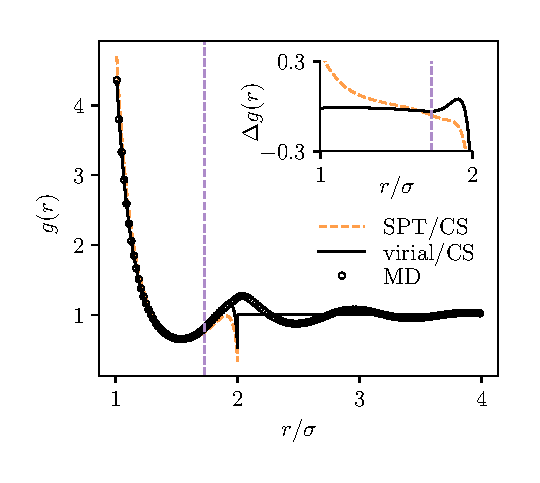
\includegraphics[width=0.9\linewidth,outer]{g2-phi045}
  \caption[Accuracy of pair distribution functions $g^{(2)}(r)$]{
    Comparing radial distribution functions of the morphometric theories with coefficients of \eqref{eq:cs-spt-coefficients} (SPT/CS), equivalent to the White Bear II in the bulk limit \cite{Hansen-GoosJPCM2006}; and \eqref{eq:virial-coefficients} with the Carnahan-Starling equation of state \eqref{eq:cs-pressure} (virial/CS), against results of molecular dynamics (MD) simulations at volume fraction $\eta = 0.45$.
    The inset shows the difference between the two theoretical distribution functions and the molecular dynamics.
    The purple dashed line indicates where the molecular surface self-intersects at $r = \sqrt{3} \sigma$, marking the end of the theory's regime of validity.}
  \label{fig:g2-full}
\end{SCfigure}

\subsection{First generalisation: SPT with an empirical equation of state}
\label{sec:cs-spt}

In the classical SPT approach described in the previous section, the SPT/PY equation of state emerges as an \emph{output} of the theory.
Taking inspiration from the White Bear free energy functional \cite{RothJPCM2002}, we reformulate the SPT argument so that the equation of state is an \emph{input} to the theory.
In so doing we aim to construct a theory from a more accurate equation of state, with the trade-off being that we must sacrifice some self-consistency.
The main equation of state we will impose is the empirical Carnahan-Starling (CS) relation \eqref{eq:cs-pressure} known to be accurate across the whole stable liquid regime \cite{CarnahanJCP1969}, and even at the high density limits accessible to simulation in the supercooled regime \cite{BerthierPRL2016} (Fig.\ \ref{fig:swap-eos}).
%The price we pay for a more accurate equation of state will be the loss of self consistency; we will no longer be able to satisfy all five of the previous equations \eqref{eq:spt-origin-continuity}, \eqref{eq:spt-mu-density-derivative} and \eqref{eq:spt-virial} simultaneously.
%Instead we must make some choice over which ones to retain.
Since the pressure is now a known input, the excess chemical potential can be determined by integrating \eqref{eq:osmotic-consistency-2} i.e.\
\begin{equation}\label{eq:excess-chemical-potential}
  \beta \mu^\mathrm{ex}[p]
  = \left( \frac{\beta p}{\rho} - 1 \right)
  + \int_0^\eta \left( \frac{\beta p}{\rho} - 1 \right) \, \frac{d\eta'}{\eta'}.
\end{equation}
To keep the expressions simple we will not evaluate the chemical potential until the very end, but it should be recognised as a known variable wherever it appears.
%% In particular, for the CS equation of state \eqref{eq:cs-pressure} this yields
%% \begin{equation}\label{eq:cs-mu}
%%   \beta \mu^\mathrm{ex} = \frac{8\eta - 9\eta^2 + 3\eta^3}{(1-\eta)^3}.
%% \end{equation}

With the pressure fixed we have three free parameters in the theory $\{a_0, a_1, a_2\}$;
we must thus choose three out of the five available thermodynamic relations in \eqref{eq:spt-origin-continuity}, \eqref{eq:spt-mu} and \eqref{eq:spt-virial} to satisfy%
\marginfootnote{Attempting to satisfy \emph{all} relations would necessarily require the previously obtained pressure \eqref{eq:py-pressure}.}.
Therefore, we must lose consistency with two of these relations to obtain a more accurate theory for practical applications.

To set the correct energy scale we choose to fix $\Delta \Omega(R=0)$ and $\Delta \Omega(R=\sigma/2)$ through equations \eqref{eq:spt-point} and \eqref{eq:spt-mu} using the chemical potential determined above in \eqref{eq:excess-chemical-potential}.
This in turn imposes the consistency of the osmotic pressure \eqref{eq:osmotic-consistency-1}.
For the final equation we choose to set the contact value of $g^{(2)}$ through \eqref{eq:spt-virial} which better represents solutes of interest than the two relations for point geometries at $R=0$.
%where the geometry is smaller than typical solutes of interest.
%occur at larger lengthscales than point insertions it makes sense to favour relations emphasising accuracy for $R \gtrsim \sigma/2$.
Solving these three equations gives the generalised SPT coefficients
% \eqref{eq:spt-point}, \eqref{eq:spt-mu} and \eqref{eq:spt-virial}
\begin{subequations}\label{eq:general-spt-coefficients}
  \begin{align}
    \beta a_0^\mathrm{SPT}
    &=
    -\frac{\ln{(1- \eta)}}{4\pi},
    \\
    \beta a_1^\mathrm{SPT}
    &=
    \frac{1}{2\pi\sigma} \left(
    (\eta - 3) \frac{\beta p}{\rho}
    + 2 \beta \mu^\mathrm{ex}[p]
    + 2 \ln{(1 - \eta)}
    + 3
    \right),
    \\
    \beta a_2^\mathrm{SPT}
    &=
    - \frac{1}{\pi \sigma^2} \left(
    (2 \eta - 3) \frac{\beta p}{\rho}
    + \beta \mu^\mathrm{ex}[p]
    + \ln{(1 - \eta)}
    + 3
    \right).
 \end{align}
\end{subequations}
It can be verified that inserting the Percus-Yevick equation of state \eqref{eq:py-pressure} into these expressions yields the previously obtained coefficients \eqref{eq:py-coefficients}, as expected.
For the CS equation of state we obtain
\begin{subequations}\label{eq:cs-spt-coefficients}
  \begin{align}
    \beta a_0^\mathrm{SPT/CS}
    &=
    -\frac{\ln{(1- \eta)}}{4\pi},
    \\
    \beta a_1^\mathrm{SPT/CS}
    &=
    \frac{1}{2\pi\sigma} \left(
    \frac{5\eta + \eta^2}{1 - \eta}
    + 2 \ln{(1 - \eta)}
    \right),
    \\
    \beta a_2^\mathrm{SPT/CS}
    &=
    \frac{1}{\pi \sigma^2} \left(
    \frac{\eta (2 + 3\eta - 2\eta^2)}{(1 - \eta)^2}
    - \ln{(1 - \eta)}
    \right),
    \\
    \frac{\beta p^\mathrm{SPT/CS}}{\rho}
    &=
    \frac{1 + \eta + \eta^2 - \eta^3}{(1-\eta)^3},
 \end{align}
\end{subequations}
which are \emph{identical} to the coefficients derived from the White Bear II (WBII) free energy functional%
\marginfootnote{We use a different normalisation of the intrinsic volumes in this chapter, so $a_1$ and $a_0$ must be multiplied through by $4\pi$ to recover \eqref{eq:wbii-coefficients}.}.
The exact form of these coefficients differs from that stated in Ref.\ \cite{Hansen-GoosJPCM2006} due to a different definition of the surface, so the equivalence only becomes clear after transforming to the excluded geometry through the canonical relations \eqref{eq:exclusion-transform}.
Remarkably, we have obtained these coefficients through a route completely different from their original derivation.

In Ref.\ \cite{Hansen-GoosJPCM2006} the coefficients were determined within FMT by taking the limit of a binary mixture where one component is infinitely dilute.
Here we completely avoided FMT, in favour of geometrical arguments similar to the classical SPT approach outlined in the previous section.
This suggests that this generalised scaled particle argument is built into the structure of the WBII functional of Ref.\ \cite{Hansen-GoosJPCM2006}; this is not an obvious fact as the derivation of this functional did not explicitly involve these arguments.
Rather, the WBII functional was constructed based on a novel extension of the CS equation to mixtures by requiring self-consistency of the pressure in \eqref{eq:osmotic-consistency-3} \cite{Hansen-GoosJCP2006}.
%The fact that these two routes lead to the same thermodynamic coefficients suggests there is an equivalence between the selected thermodynamic relations.
We imposed this relation by setting the chemical potential in \eqref{eq:spt-mu} using the chemical potential obtained via \eqref{eq:osmotic-consistency-2}.
It is unclear to us how our final choice of using \eqref{eq:spt-mu} instead of one of the two relations at the origin, i.e.\ \eqref{eq:spt-point-d1} or \eqref{eq:spt-point-d2}, is built into the WBII functional.

Finally, note that the resulting $g^{(2)}$ obtained from direct evaluation of the potential of mean force \eqref{eq:potential-mean-force} with the SPT/CS coefficients performs poorly in the supercooled regime compared with the ``exact'' result from the virial theorem i.e.\ equation \eqref{eq:contact-g}.
To demonstrate this we plot the contact value in Fig.\ \ref{fig:contact-g} for this set of coefficients, finding that it is reasonably accurate until around the freezing density where contact correlations spuriously decay.
The next section will detail how to modify this argument to produce coefficients which describe more accurate correlation functions at high densities.

\begin{SCfigure}
  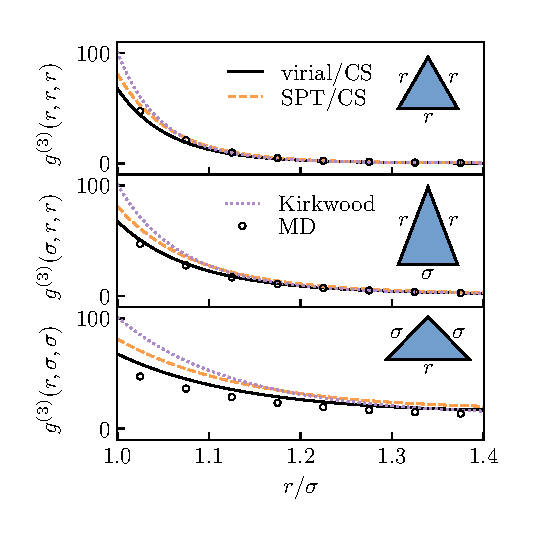
\includegraphics[width=0.9\linewidth,outer]{g3}
  \caption[Accuracy of triplet distribution functions $g^{(3)}(r,s,t)$]{
    Comparison of predicted correlations for triangular geometries against molecular dynamics simulations at volume fraction $\eta = 0.45$.}
  \label{fig:g3}
\end{SCfigure}

\subsection{Second generalisation: self-consistency of the contact value of $g^{(2)}(r)$ with the virial theorem}
\label{sec:virial-spt}

Our goal is to develop a morphometric theory which produces accurate correlation functions $g^{(n)}$.
As described at the end of the last section, the correlation functions produced by an SPT approach are inaccurate at high densities.
We will correct the spurious decay of the contact value of the pair distribution function $g^{(2)}(r)$ at high densities by building this into the theory explicitly, with the aim of producing more accurate correlation functions.

%% This represents a significant departure from strictly scaled particle arguments, 
%% The great strength of the morphometric approach over scaled particle arguments is that we are not restricted to purely rescaling; in principle the form should be valid for arbitrary geometries.
%% We can use this strength of the morphometric approach to construct a new theory which satisfies the virial theorem.}

The potential of mean force \eqref{eq:potential-mean-force} for non-overlapping spheres with the morphometric \emph{ansatz} \eqref{eq:morph-ansatz} is written
\begin{equation}\label{eq:phi2}
  \begin{split}
    \phi^{(2)}(r)
    :=&
    - k_B T \ln g^{(2)}(r)
    \\ =&
    p V_3(r) + a_2 A (r) + a_1 C(r) + a_0 X(r) - 2\mu^\mathrm{ex}[p]
  \end{split}
\end{equation}
so we need the size measures for the two particle solute resembling a ``dumbbell''.
It is easier to calculate the excluded volume geometry, after which we can obtain the molecular volumes using the canonical relations given in e.g.\ Ref.\ \cite{OettelEL2009}.
The excluded volume consists of the union of two balls of radius $\sigma$ separated by a distance $r$.
The geometric properties at contact are then \cite{OettelEL2009}
\begin{align*}
  X_+(\sigma)
  &=
  4 \pi
  \\
  C_+(\sigma)
  &=
  \left( 6 - \frac{\pi}{2\sqrt{3}} \right) \pi \sigma,
  \\
  A_+(\sigma)
  &=
  6 \pi \sigma^2,
  \\
  V_+(\sigma)
  &=
  \frac{9 \pi \sigma^3}{4}.
\end{align*}
Transforming to the parallel molecular surface using the inverse transformation of \eqref{eq:exclusion-transform-volumes} gives the solute parameters as
\begin{subequations}
  \begin{align}
    C(\sigma)
    &=
    \left( 4 - \frac{\pi}{2\sqrt{3}} \right) \pi \sigma,
    \\
    A(\sigma)
    &=
    \left( 1 + \frac{\pi}{2\sqrt{3}} \right) \pi \sigma^2,
    \\
    V(\sigma)
    &=
    \left( \frac{7}{12} - \frac{\pi}{8\sqrt{3}} \right) \pi \sigma^3.
  \end{align}
\end{subequations}
Inserting these volumes into \eqref{eq:phi2} and applying the virial theorem \eqref{eq:contact-g} for the contact value of $g^{(2)}$ gives the final expression
\begin{align}\label{eq:v-virial}
  &
  p \left( \frac{7}{12} - \frac{\pi}{8\sqrt{3}} \right) \pi \sigma^3
  + a_2 \left( 1 + \frac{\pi}{2\sqrt{3}} \right) \pi \sigma^2
  + a_1 \left( 4 - \frac{\pi}{2\sqrt{3}} \right) \pi \sigma
  + a_0 \, 4\pi
  \nonumber \\ = \; &
  2\mu^\mathrm{ex}[p] - \beta^{-1} \ln{\frac{3}{2\pi \rho \sigma^3} \left( \frac{\beta p}{\rho} - 1 \right)}.
\end{align}
We will use this last expression instead of the contact theorem \eqref{eq:spt-virial} in order to obtain new coefficients.
Together \eqref{eq:spt-point}, \eqref{eq:spt-mu} and \eqref{eq:v-virial} solve to give coefficients:
\begin{subequations}\label{eq:virial-coefficients}
  \begin{align}
    \beta a_0^\mathrm{virial}
    &=
    -\frac{\ln{(1- \eta)}}{4\pi},
    \\
    \beta a_1^\mathrm{virial}
    &=
    \frac{1}{(\sqrt{3}\pi - 4)\pi\sigma}
    \left[
    \vphantom{\ln{\left( \frac{\frac{\beta p}{\rho} - 1 }{4\eta} \right)}}
    \left(5 - \frac{5\pi}{2\sqrt{3}}\right)
    \eta \frac{\beta p}{\rho}
    - \left( 2 - \frac{\pi}{\sqrt{3}} \right) \beta \mu^\mathrm{ex}[p]
    \right.
    \nonumber \\
    & \qquad \qquad \qquad \qquad
    \left.
    + \frac{\pi}{\sqrt{3}} \ln{(1 - \eta)}
    + 2 \ln{\left( \frac{\frac{\beta p}{\rho} - 1 }{4\eta} \right)}
    \right],
    \\
    \beta a_2^\mathrm{virial}
    &=
    - \frac{1}{(\sqrt{3}\pi - 4)\pi \sigma^2}
    \left[
    \vphantom{\ln{\left( \frac{\frac{\beta p}{\rho} - 1 }{4\eta} \right)}}
    \left(6 - \frac{2\pi}{\sqrt{3}}\right)
    \eta \frac{\beta p}{\rho}
    - \frac{\pi}{\sqrt{3}} \beta \mu^\mathrm{ex}[p]
    \right.
    \nonumber \\
    & \qquad \qquad \qquad
    \left.
    + \left( 4 - \frac{\pi}{\sqrt{3}} \right) \ln{(1 - \eta)}
    + 4 \ln{\left( \frac{\frac{\beta p}{\rho} - 1 }{4\eta} \right)}
    \right].
 \end{align}
\end{subequations}
We refer to coefficients obtained this way for the CS pressure \eqref{eq:cs-pressure} as virial/CS, but we will not give them explicitly.
Unlike the WBII coefficients above these are new.
The pair correlation produced by these coefficients (black line in Fig.\ \ref{fig:contact-g}) is self-consistent with CS at contact by construction.

\begin{SCfigure}
  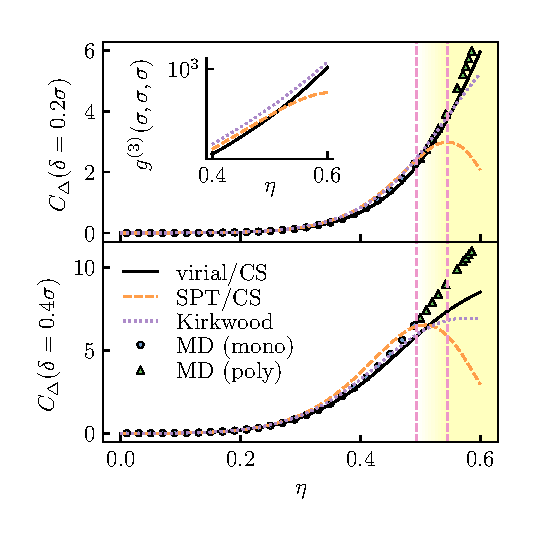
\includegraphics[width=0.9\linewidth,outer]{sp3}
  \caption[Number of triangles in the bulk liquid]{
    Concentration of triangles in the hard sphere liquid with side lengths $r,s,t \in [\sigma, \sigma + \delta]$ versus volume fraction.
    Direct measurements by molecular dynamics using a single-component system and an 8\% polydisperse system, while the lines show predictions from the morphometric theories described in text.
    The hard sphere freezing and melting volume fractions are indicated by pink dashed lines to show the onset of the supercooled regime.
    Inset: contact value of $g^{(3)}$ showing how the errors in the SPT/CS theory arise from underestimation close to contact.}
  \label{fig:sp3}
\end{SCfigure}

\begin{SCfigure}
  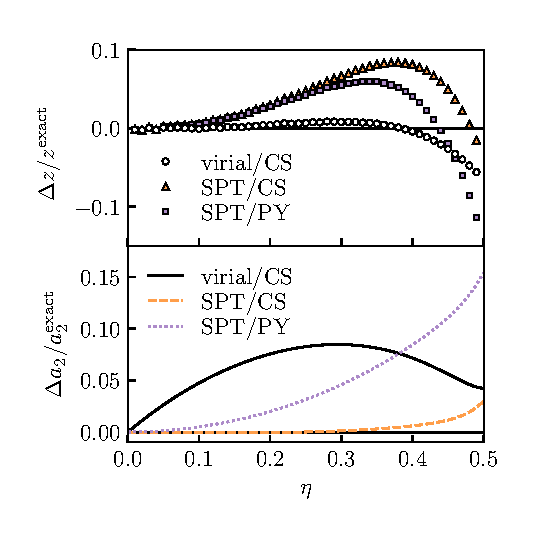
\includegraphics[width=0.9\linewidth,outer]{a2-errors}
  \caption[Comparing of theoretical surface tensions against literature values]{
    Errors in different morphometric theories for hard spheres.
    Top panel: error in the coordination defined in \eqref{eq:coordination}, giving the average number of neighbours in the shell $r < 1.4\sigma$ around a particle.
    Bottom panel: planar surface tensions against volume fraction, using the highly accurate result \eqref{eq:quasi-exact-surface-tension} from Ref.\ \cite{DavidchackMP2015} valid until $\eta \sim 0.5$.
  The theories compared are virial/CS, new coefficients given in \eqref{eq:virial-coefficients}; SPT/CS, equivalent to the White Bear II \cite{Hansen-GoosJPCM2006} given in \eqref{eq:cs-spt-coefficients}; and SPT/PY, the classical scaled particle theory \cite{ReissJCP1959} given in \eqref{eq:py-coefficients}.}
  \label{fig:surface-tension}
\end{SCfigure}

\section{Numerical results}
\label{sec:numerics}

We apply the thermodynamic coefficients determined in previous sections for a system of hard spheres to obtain two-- and three--body distribution functions using the generlaised potential of mean force \eqref{eq:potential-mean-force} with the morphometric approach \eqref{eq:morph-ansatz}, and compare these against molecular dynamics simulations.
For the analytics we determine the input geometric quantities $\{V,A,C,X\}$ using the algorithms of Refs.\ \cite{MeckeAA1994,KleninJCC2011}.
For the simulations we performed event-driven molecular dynamics of $N=1372$ monodisperse hard spheres using the DynamO software package \cite{BannermanJCP2010}.
We measure the pair and triplet distribution functions $g^{(2)}$ and $g^{(3)}$ for simulations at $\eta = 0.45$.
For simulations above freezing $\eta \simeq 0.494$ we used a 5-component equimolar distribution with $\sim8\%$ polydispersity.

For $g^{(2)}$ shown in Fig.\ \ref{fig:g2-full} we find the virial/CS theory outperforms the SPT/CS theory even away from contact.
The agreement with the molecular dynamics simulations is excellent, until $r \gtrsim \sqrt{3}\sigma$ where the solute boundary self-intersects and outside the regime of the theory's validity (see discussion in Ref.\ \cite{OettelEL2009}).
The physical interpretation of this breakdown is that for $r > \sqrt{3}\sigma$ interactions between solvent particles can occur \emph{through} the solute, so these correlations will not be captured by the theory.
Only the contact value was fixed, so accuracy for $r > \sigma$ was not guaranteed; the accuracy is a welcome bonus.
We can quantify this accuracy through the integrated value
\begin{equation}\label{eq:coordination}
  z(\delta)
  =
  4\pi \int_\sigma^{\sigma+\delta}
  \rho^{(2)}(r) \, r^2 \, dr
\end{equation}
shown in the top panel of Fig.\ \ref{fig:surface-tension} where we take $\delta = 0.4\sigma$.

Now we look at the three-body correlation functions.
Triplet geometries are characterised by a triangle of side lengths $r,s,t$ so $g^{(3)} = g^{(3)}(r,s,t)$.
We also compare the morphometric theories against the Kirkwood approximation \cite{KirkwoodJCP1935} i.e.\
\begin{equation}
  g^{(3)}(r, s, t)
  \approx
  g^{(2)}(r) g^{(2)}(s) g^{(2)}(t)
\end{equation}
where we take the values of $g^{(2)}$ from the virial/CS theory because of its already demonstrated accuracy at the two body level.
Comparison of the morphometric correlation functions, including with the Kirkwood closure, against molecular dynamics are shown in Fig.\ \ref{fig:g3}.
The virial/CS closure most closely matches the simulations at high densities, suggesting the theory is suitable for modeling complex many-particle local structures \cite{RobinsonPRL2019}.
To illustrate this we consider the concentration of triangles with side lengths $r,s,t \in [\sigma, \sigma + \delta]$ in the bulk liquid, from \eqref{eq:n-particle-density-pdf} we find this as%
\marginfootnote{We state the measure here without proof, though we present a general method to obtain this (at least numerically) for arbitrary $n$ in the next chapter.
  The analytic form $rst \, dr ds dt$ for the specific three-body case is presented in e.g.\ Ref.\ \cite{KrumhanslJCP1972}.}
\begin{equation}
  C_\Delta(\delta)
  =
  8\pi^2 \int_\sigma^{\sigma+\delta}\int_\sigma^{\sigma+\delta}\int_\sigma^{\sigma+\delta}
  %e^{-\beta\phi^{(3)}
  \rho^{(3)}(r,s,t) \, rst \, dr ds dt.
\end{equation}
Comparison of this quantity against molecular dynamics simulations shows similar levels of accuracy for small $\delta$, though the performance decreases as it is increased above the first minimum of the $g^{(2)}(r)$; this is not surprising as our virial closure emphasised accuracy at contact.
Notably, the Kirkwood approximation performs surprisingly well at the three-body level in both of these tests.

Next we compare the theories' predicted surface tension against simulation data.
The surface tension at a planar wall is simply $a_2$ because it conjugates with the area.
In Ref.\ \cite{DavidchackMP2015} a highly accurate $a_2$ was measured for hard spheres through extensive simulation, which was parameterised by the following expression
\begin{equation}\label{eq:quasi-exact-surface-tension}
  %\begin{split}
  \beta a_2
  =
  \frac{1}{\pi \sigma^2} \left(
  \frac{\eta (2 + 3\eta - \frac{9}{5}\eta^2 - \frac{4}{5}\eta^3 - (5 \times 10^4) \eta^{20})}{(1 - \eta)^2}
  %% \right.
  %% \\
  %% &
  %% \left.
  %% \vphantom{\frac{1}{1}}
  - \ln{(1 - \eta)}
  \right).
  %\end{split}
\end{equation}
Comparing this highly accurate expression against the values predicted from the morphometric coefficients, we find the virial/CS surface tension is less accurate than the SPT/CS prediction (Fig.\ \ref{fig:surface-tension}) despite its superior correlation functions at high densities.
One of the great strengths of the SPT/CS theory is its accuracy in the planar limit \cite{Hansen-GoosJPCM2006}, so this suggests that the virial/CS theory sacrifices asymptotic accuracy for more self-consistency in the correlation functions.
For this reason, SPT/CS coefficients may give more accurate grand potentials (and thus correlations) for large solutes where the surface becomes approximately planar.

\section{Conclusions}

We have presented the morphometric approach as a generalisation of SPT, thus placing the scaled particle \emph{ansatz} on more precise and physically motivated assumptions i.e.\ those underlying the theorems of integral geometry.
Using the scaled particle approach we have systematically derived several theories for the hard sphere liquid.
This included the classical SPT solution and the morphometric theory obtained in the bulk limit of free energy functionals based on the CS equation of state%
\marginfootnote{See the discussion around \eqref{eq:wbii-coefficients} in section \ref{sec:fmt} for details of the original derivation.},
although our method of deriving the latter theory is new.
The third theory we derived is particularly suited for treating many-body correlations, which we used to accurately treat local structures in the hard sphere liquid in Ref.\ \cite{RobinsonPRL2019}.

By making the underlying assumptions explicit we can better understand the limits of the theory: any deviation from the morphometric/SPT \emph{ansatz} must be due to a violation of translation/rotation invariance, additivity or continuity.
The fact that these theories are very accurate for hard spheres suggests that the assumptions are only weakly violated for this system.
While translational/rotational invariance and continuity are physically plausible conditions on $\Delta \Omega$, additivity is a very strong assumption.
In particular, we expect significant deviations from additivity where the liquid develops a static length scale exceeding the size of the solute \cite{KonigPRL2004}.
As such, we expect the validity of the morphometric approach to require the solute to be larger than the point-to-set length \cite{MontanariJSP2006}, which acts as an upper bound for all structural length scales \cite{YaidaPRE2016}.
The morphometric \emph{ansatz} must break down approaching a critical point, so it cannot be used to obtain asymptotics in the event of a thermodynamic glass transition.

Finally, we remark that while it is tempting to call the treatment of bulk degrees of freedom with the morphometric approach mean-field, this is not a completely accurate characterisation.
Mean-field theories typically become formally exact in the limit of infinite spatial dimensions, where the thermodynamic role of fluctuations disappears.
By contrast, the morphometric approach (and related theories like SPT and FMT) become formally exact in the one-dimensional limit of hard rods%
\marginfootnote{We will discuss this limit in more detail in chapter \ref{chapter:resummation}.}.
Though this theory does not explicitly describe fluctuations, they are built into the choice of thermodynamic coefficients entering the theory.
In this sense it is more accurate to describe the morphometric approach (and related theories) as an \emph{excluded volume} theory, or as a \emph{free volume} theory because the thermodynamics only shows divergent behaviour as $\eta \to 1$.

%Possible other things to mention:
%\begin{itemize}
%%   \item We have obtained these morphometric theories independent of FMT, though we the two theories are intimately related.
%% In particular, they are both rooted in ideas of integral geometry and morphometry is obtained as a limit case of FMT.
%The morphometric approach enables much more 
%\item
%As a model for depletion interactions it generalises and supercedes earlier theories like the Asakura-Oosawa model or its extensions using the Derjaguin approximation \cite{OettelEL2009}.
%\end{itemize}

\ifdefined\includebibliography
  \printbibliography
\fi

\end{document}
